% !TEX program = xelatex
\documentclass[12pt, a4paper]{article}
\usepackage[margin=1in]{geometry}
\usepackage{xeCJK}
\setCJKmainfont{SimSun} % 设置中文字体
\setmainfont{Times New Roman} % 设置英文字体
\usepackage{amsmath, amssymb}
\usepackage{graphicx}
\usepackage{booktabs}
\usepackage{hyperref}
\usepackage{setspace}
\usepackage{listings}
\usepackage{tikz}
\usetikzlibrary{positioning}
\usepackage{color}
\usepackage{float}

% 代码块设置
\definecolor{dkgreen}{rgb}{0,0.6,0}
\definecolor{gray}{rgb}{0.5,0.5,0.5}
\definecolor{mauve}{rgb}{0.58,0,0.82}
\lstset{frame=tb,
  language=Python,
  aboveskip=3mm,
  belowskip=3mm,
  showstringspaces=false,
  columns=flexible,
  basicstyle={\small\ttfamily},
  numbers=none,
  numberstyle=\tiny\color{gray},
  keywordstyle=\color{blue},
  commentstyle=\color{dkgreen},
  stringstyle=\color{mauve},
  breaklines=true,
  breakatwhitespace=true,
  tabsize=3
}

\hypersetup{colorlinks=true, linkcolor=blue, urlcolor=blue}
\onehalfspacing

\title{学校社会资本对初中生教育期望的影响:\\基于 CEPS 数据的实证分析与复现报告}
\author{分析员:Lucian Lin}
\date{\today}

\begin{document}

\maketitle

\begin{abstract}
本研究基于 CEPS 第二轮数据(有效样本≈9k,排除“10=无所谓”),构建有序 Logit 并使用班级聚类稳健 SE,检验学校社会资本对教育期望的作用。事前假设为“补偿效应”:Linking/Bonding 对弱势(低 SES、农村)更有帮助。实证结果显示:主效应均显著正向;Bonding×SES 为正(高 SES 获益更多,趋势性 p≈0.052);Linking×SES 不显著;Linking×Rural 正向但未显著。PO 假设被拒绝(与多项 Logit 对比),Linking 存在非线性信号(样条 p≈0.005)。报告提供变量构造(PCA-SES、Bonding/Linking)、问卷选项表、交互/非线性图,以及复现实录,便于后续研究对照与扩展。
\end{abstract}

\section{研究目标与假设 (Research Objectives)}

教育期望(Educational Expectations)是预测青少年未来教育获得与社会分层的关键心理代理变量。本研究聚焦学校场域的社会资本,事前假设为“补偿效应”,即弱势群体从学校社会资本中获益更多。具体假设:
\begin{itemize}
    \item \textbf{H1(主效应)}:Teacher Linking 与 Peer Bonding 均正向预测教育期望(控制 SES、户籍、认知)。
    \item \textbf{H2(补偿效应)}:
    \begin{itemize}
        \item H2a:Linking 对低 SES 学生的正向作用强于高 SES(Linking $\times$ SES $<0$)。
        \item H2b:Bonding 对低 SES 学生的正向作用强于高 SES(Bonding $\times$ SES $<0$)。
        \item H2c:Linking 对农村户籍学生的正向作用强于城市户籍(Linking $\times$ Rural $>0$)。
    \end{itemize}
    \item \textbf{H3(探索性)}:比较两种学校社会资本对弱势群体的“补偿力度”——检验 Teacher Linking 是否比 Peer Bonding 更能提升低 SES/农村学生(或至少不产生优势累积)。
\end{itemize}

\section{数据来源与样本清洗 (Data \& Sample)}

\subsection{数据源}
本研究使用 \textbf{CEPS Wave 2}(八年级追踪数据)。该数据具有全国代表性,采用多阶段概率与规模成比例(PPS)抽样。

\subsection{样本筛选与处理}
原始样本量约为 9,400 人。针对因变量 \texttt{expect\_edu\_raw} 的特殊编码进行如下处理:
\begin{itemize}
    \item \textbf{剔除 ``10=无所谓''}:在有序回归框架下,“无所谓”无法简单定序为最高或最低。本研究将其视为非随机缺失剔除(Listwise Deletion),最终分析样本 $N \approx 9,012$。
    \item \textbf{局限性说明}:若“无所谓”群体具有系统性偏差(如多为低成绩学生),直接剔除可能导致估计有偏,后续建议通过 Heckman 选择模型或多项 Logit 进行稳健性检验。
    \item \textbf{聚类变量}:保留班级 ID (\texttt{clsids}) 用于计算聚类稳健标准误(Cluster-Robust Standard Errors),以校正班级内部的扰动项相关性。
\end{itemize}

\section{变量构造与测度 (Variable Construction)}

为确保可复现性,所有连续变量在合成后均进行了 Z-score 标准化(Mean=0, SD=1)。

\paragraph{概念定义(含英文出处,便于写作与引用)}
\begin{itemize}
    \item \textbf{Bonding social capital}(同伴/组内纽带):密集、同质的强关系(亲友/同班/同圈层),强化组内互助与凝聚力。典型定义:Putnam, 2000; Szreter \& Woolcock, 2004.
    \item \textbf{Linking social capital}(纵向/与权威的联结):跨越正式权力层级,连接制度性资源或权威者(如教师、官员、服务提供者),用于获取信息与支持。典型定义:Woolcock, 2001; Szreter \& Woolcock, 2004.
    \item (对照)\textit{Bridging} = 横向异质连接,本文非核心,但可用于解释同伴结构的异质性。
\end{itemize}

\subsection{因变量:教育期望}
\begin{itemize}
    \item \textbf{变量名}:\texttt{expect\_edu\_raw}
    \item \textbf{定义}:保留 1-9 的有序分类(1=不读了/小学,...,9=博士)。
    \item \textbf{清洗规则}:\texttt{value == 10} $\rightarrow$ \texttt{NaN}。
\end{itemize}

\begin{table}[H]
\centering
\caption{教育期望(w2b18)原题与选项映射}
\label{tab:expectation_codes}
\begin{tabular}{cll}
\toprule
代码 & 中文选项 & English description \\
\midrule
1 & 不念了/现在就不要念了 & Stop schooling now \\
2 & 初中毕业 & Junior middle school \\
3 & 中专/技校 & Vocational/technical secondary \\
4 & 职业高中 & Vocational high school \\
5 & 普通高中 & Academic high school \\
6 & 大学专科(大专/高职) & College diploma/associate \\
7 & 大学本科 & Bachelor’s degree \\
8 & 研究生(硕士) & Master’s degree \\
9 & 博士 & Doctorate \\
10* & 无所谓/没有具体打算 & Doesn’t matter (excluded from ordered model) \\
\bottomrule
\end{tabular}
\vspace{0.5em}
\footnotesize{* 代码 10 仅用于描述原问卷,已在有序模型中剔除;分析样本为 1–9。}
\end{table}

\subsection{核心自变量:学校社会资本}
\begin{enumerate}
    \item \textbf{同伴纽带 (Bonding)}:
    \begin{itemize}
        \item \textbf{源变量}:\texttt{w2b0605}(经常有麻烦)、\texttt{w2b0606}(同学友善)、\texttt{w2b0607}(归属感)。
        \item \textbf{计算}:先对 \texttt{w2b0605} 进行反向计分,然后计算三者的均值(或加总)。
        \item \textbf{标准化}:$Bonding = (X - \bar{X}) / \sigma_X$。
    \end{itemize}
    \item \textbf{师生联结 (Linking)}:
    \begin{itemize}
        \item \textbf{维度 A(表扬)}:\texttt{teacher\_praise} = Mean(\texttt{w2b0507}, \texttt{w2b0508}, \texttt{w2b0509})(主课老师表扬频率)。
        \item \textbf{维度 B(互动)}:\texttt{teacher\_talk} = 源自 \texttt{w2c09}(是否经常主动与老师谈话)。编码规则:\texttt{1} (经常) $\rightarrow$ 1, \texttt{2/3/4} (偶尔/从不) $\rightarrow$ 0。
        \item \textbf{合成}:$Linking_{raw} = Z(teacher\_praise) + Z(teacher\_talk)$,最后再次 Z-score 标准化。
    \end{itemize}
\end{enumerate}

\paragraph{问卷题目与选项(完整呈现)}
\begin{table}[H]
\centering
\caption{Bonding \& Linking 题目及选项编码(频率 1--4 递增)}
\label{tab:items_bond_link}
\begin{tabular}{p{2.5cm}p{5.3cm}p{5.5cm}}
\toprule
变量 & 题目(中文简述) & 选项编码(CEPS 频率制) \\
\midrule
w2b0605 & 经常有麻烦 / 遭同学欺负 & 1=从不,2=偶尔,3=有时,4=经常(反向计分) \\
w2b0606 & 同学对我很友善 & 1=从不,2=偶尔,3=有时,4=经常 \\
w2b0607 & 我觉得自己是班级一分子(归属感) & 1=从不,2=偶尔,3=有时,4=经常 \\
w2b0507 & 主课老师在课堂上表扬我 & 1=从不,2=偶尔,3=经常,4=总是 \\
w2b0508 & 主课老师课后表扬我 & 1=从不,2=偶尔,3=经常,4=总是 \\
w2b0509 & 当我表现好时老师会表扬我 & 1=从不,2=偶尔,3=经常,4=总是 \\
w2c09   & 你是否经常主动与老师谈话 & 1=经常,2=有时,3=很少,4=从不(本研究:1$\rightarrow$1;2/3/4$\rightarrow$0) \\
\bottomrule
\end{tabular}
\vspace{0.4em}
\footnotesize{所有条目原始取值均为 1--4 递增频率,除 w2c09 另行二元化;w2b0605 反向计分后再参与合成。}
\end{table}

\subsection{调节变量:家庭社会经济地位 (SES) - PCA 方法}
采用主成分分析(Principal Component Analysis, PCA)构建综合 SES 指标,以避免多重共线性。

\subsubsection{什么是 PCA?——用"综合评分"的比喻来理解}
假设你想评价一个家庭的社会经济地位,手上有 5 个指标:父母学历、家庭经济、藏书量、是否有书桌、是否有电脑。这些指标彼此相关(有钱的家庭往往藏书也多),直接放入回归会产生\textbf{多重共线性}问题。

PCA 的思路是:找到一个"综合评分",用一个数字概括这 5 个指标的共同信息。具体步骤如下:

\begin{enumerate}
    \item \textbf{标准化}:把每个指标转换为均值为 0、标准差为 1 的形式,消除量纲差异
    \item \textbf{计算相关性}:看这 5 个指标之间的相关程度(图 \ref{fig:pca_input_corr})
    \item \textbf{提取主成分}:找到能最大程度概括原始信息的"方向"(数学上是特征向量)
    \item \textbf{选择保留几个}:通过碎石图(图 \ref{fig:pca_scree})判断,通常选择"拐点"之前的成分
    \item \textbf{计算得分}:用保留的主成分给每个学生打分
\end{enumerate}

\subsubsection{投入指标}
SES 指标由以下 5 个问卷条目构建:

\begin{table}[H]
\centering
\caption{SES 主成分分析投入变量及编码}
\label{tab:ses_items}
\begin{tabular}{p{2.8cm}p{4.5cm}p{5.5cm}}
\toprule
变量来源 & 题目简述 & 选项编码 \\
\midrule
w2a10/w2a11 & 父/母受教育程度(取最高值) & 1=没受过任何教育,2=小学,3=初中,4=中专/技校,5=职业高中,6=普通高中,7=大专,8=本科,9=研究生及以上 \\
w2a09 & 家庭经济状况自评 & 1=非常困难,2=比较困难,3=中等,4=比较富裕,5=很富裕 \\
w2a13 & 家中藏书量 & 1=没有,2=1--10本,3=11--25本,4=26--100本,5=101--200本,6=201--500本,7=500本以上 \\
w2a1401 & 是否有独立书桌 & 1=有,0=没有(原编码反向处理) \\
w2a1402 & 是否有独立电脑 & 1=有,0=没有(原编码反向处理) \\
\bottomrule
\end{tabular}
\vspace{0.4em}

\footnotesize{\textit{注}:所有变量先标准化(Z-score),再投入 PCA;提取第一主成分(PC1)作为综合 SES 得分。}
\end{table}

\subsubsection{PCA 结果可视化}

图 \ref{fig:pca_scree} 是\textbf{碎石图},展示每个主成分解释了多少原始方差。可以看到:
\begin{itemize}
    \item PC1(第一主成分)解释了 44.1\% 的方差,远高于其他成分
    \item PC2 之后的成分解释力急剧下降("拐点"出现在 PC1 之后)
    \item 因此,我们只保留 PC1 作为 SES 的综合指标
\end{itemize}

\begin{figure}[H]
  \centering
  \includegraphics[width=0.8\textwidth]{../figures/report_phase3/pca_scree_plot.png}
  \caption{碎石图:PC1 解释了 44.1\% 的方差,是主要的"综合评分"维度。橙色折线显示累计解释方差。}
  \label{fig:pca_scree}
\end{figure}

图 \ref{fig:pca_loadings} 展示了 PC1 的\textbf{载荷}(Loading),即每个原始变量对 PC1 的贡献权重:
\begin{itemize}
    \item 所有载荷都是正值,说明 PC1 确实是一个"综合 SES"指标
    \item 家庭藏书(0.511)和有书桌(0.486)贡献最大——这些是文化资本的体现
    \item 父母学历(0.458)和家庭经济(0.419)次之
    \item 有电脑(0.343)贡献最小,可能因为电脑在当代中国已较为普及
\end{itemize}

\begin{figure}[H]
  \centering
  \includegraphics[width=0.8\textwidth]{../figures/report_phase3/pca_loadings.png}
  \caption{PC1 载荷:所有变量都正向贡献于 SES 综合得分,藏书和书桌权重最高。}
  \label{fig:pca_loadings}
\end{figure}

图 \ref{fig:pca_ses_dist} 展示了最终 SES 得分的分布。得分越高代表家庭社会经济地位越好。

\begin{figure}[H]
  \centering
  \includegraphics[width=0.8\textwidth]{../figures/report_phase3/pca_ses_distribution.png}
  \caption{SES 得分分布:呈近似正态分布,均值为 0,中位数为 0.18。}
  \label{fig:pca_ses_dist}
\end{figure}

\begin{figure}[H]
  \centering
  \includegraphics[width=0.7\textwidth]{../figures/report_phase3/pca_input_correlation.png}
  \caption{SES 输入变量相关矩阵:5 个指标之间存在中度正相关,适合用 PCA 降维。}
  \label{fig:pca_input_corr}
\end{figure}

\subsection{控制变量}

\begin{table}[H]
\centering
\caption{控制变量定义与编码}
\label{tab:control_vars}
\begin{tabular}{p{2.5cm}p{3.5cm}p{6.5cm}}
\toprule
变量 & 来源/定义 & 选项编码与处理 \\
\midrule
Hukou(户籍) & w2a18「你现在的户口登记地是?」 & 1=农业户口 $\rightarrow$ 1(农村);2=非农业户口 $\rightarrow$ 0(城镇);3=居民户口(已取消区分) $\rightarrow$ 0;4=不清楚 $\rightarrow$ 缺失 \\
Cognitive(认知) & w2cogscore(CEPS 标准化认知测试得分) & 连续变量,范围约 --3 至 +3;0 分视为缺考/异常剔除;其余 Z-score 标准化 \\
\bottomrule
\end{tabular}
\end{table}

\noindent\textbf{缺失值处理}:对于控制变量的少量缺失($<5\%$),采用班级均值(连续变量)或众数(分类变量)填补。

\section{统计模型与公式 (Statistical Models)}

\subsection{Ordered Logit Model}
鉴于因变量 $Y$ 为定序变量,采用 Ordered Logit 模型。假设存在一个潜在连续变量 $Y^*$:
\begin{equation}
Y^*_i = x_i'\beta + \epsilon_i, \quad \epsilon_i \sim Logistic(0, \frac{\pi^2}{3})
\end{equation}
观测到的 $Y_i$ 由一系列切点(Cut-points)$\theta_k$ 决定:
\begin{equation}
Y_i = k \quad \text{if } \theta_{k-1} < Y^*_i \le \theta_k
\end{equation}
累积概率公式为:
\begin{equation}
P(Y_i \le k | x_i) = \Lambda(\theta_k - x_i'\beta) = \frac{1}{1 + \exp(-(\theta_k - x_i'\beta))}
\end{equation}
其中,$k=1, 2, \dots, 8$(针对 9 个类别)。

\subsection{交互效应模型}
为检验调节效应,模型中加入交互项:
\begin{equation}
\text{Logit}(P(Y \le k)) = \theta_k - (\beta_1 Bonding + \beta_2 SES + \beta_3 (Bonding \times SES) + \dots)
\end{equation}
若 $\beta_3 > 0$,表明 SES 越高,Bonding 对教育期望的正向影响越大(马太效应)。

\subsection{比例优势假设 (Proportional Odds Assumption) 检验}
Ordered Logit 假设自变量对不同阈值(如“上高中”vs“上大学”)的影响系数 $\beta$ 是恒定的。本研究将使用 Brant Test 或似然比检验(Likelihood Ratio Test)对比 Ordered Logit 与 Multinomial Logit。若 PO 假设被拒绝($p < 0.05$),意味着系数存在异质性,结果解释需谨慎。

\section{结果与可视化 (Results \& Visualization)}

\subsection{描述性统计}

\subsubsection{因变量分布}
图 \ref{fig:dist} 展示了因变量的分布情况。可以看出,数据存在明显的左偏(Left-skewed)趋势,绝大多数学生期望获得本科及以上学历。其中,选择"本科"(代码 7)的学生最多,约占 37\%;其次是"硕士"和"大专"。这反映了当代中国初中生普遍较高的教育期望。

\begin{figure}[H]
  \centering
  \includegraphics[width=0.8\textwidth]{../figures/report_phase3/expectation_distribution.png}
  \caption{教育期望分布(1--9,已剔除"无所谓"选项)}
  \label{fig:dist}
\end{figure}

\subsubsection{核心自变量分布}
图 \ref{fig:dist_bonding} 和图 \ref{fig:dist_linking} 分别展示了两个核心自变量——同伴关系(Bonding)和师生关系(Linking)的分布。两者均经过标准化处理(均值为 0),呈现多峰分布特征,这是由于原始问卷采用离散选项(如"非常同意"到"非常不同意")导致的。

\begin{figure}[H]
  \centering
  \includegraphics[width=0.75\textwidth]{../figures/report_phase3/dist_bonding_idx.png}
  \caption{同伴关系指数(Bonding)分布:衡量学生与同班同学的关系质量,包括是否经常遇到麻烦、同学是否友善、是否有归属感三个维度。}
  \label{fig:dist_bonding}
\end{figure}

\begin{figure}[H]
  \centering
  \includegraphics[width=0.75\textwidth]{../figures/report_phase3/dist_linking_idx.png}
  \caption{师生关系指数(Linking)分布:衡量学生与老师的互动质量,包括老师表扬频率和主动与老师交流的意愿两个维度。}
  \label{fig:dist_linking}
\end{figure}

\subsubsection{变量间相关性}
图 \ref{fig:corr} 展示了核心变量之间的相关系数矩阵。几个值得注意的发现:
\begin{itemize}
    \item \textbf{Bonding 与 Linking 中度相关}($r=0.46$):说明在学校人际关系好的学生,往往同伴关系和师生关系都较好,但两者并非完全重叠,可以作为独立变量纳入模型。
    \item \textbf{认知能力与教育期望相关最强}($r=0.30$):学业成绩好的学生对未来有更高期望。
    \item \textbf{户籍与其他变量弱负相关}:农村学生的社会资本、SES 和认知得分略低于城市学生。
\end{itemize}

\begin{figure}[H]
  \centering
  \includegraphics[width=0.8\textwidth]{../figures/report_phase3/correlation_matrix.png}
  \caption{核心变量相关系数矩阵:颜色越红表示正相关越强,越蓝表示负相关越强。对角线为 1(自身相关)。}
  \label{fig:corr}
\end{figure}

\subsection{回归结果 (Regression Coefficients)}
基于 Python \texttt{statsmodels} 的拟合结果(Cluster by \texttt{clsids}):

\begin{table}[H]
\centering
\caption{Ordered Logit Model Results (Selected)}
\begin{tabular}{lcccc}
\toprule
Variable & Coeff (Log-Odds) & Std. Err. & P-value & 解释 \\
\midrule
\textbf{Linking} & 0.19 & 0.02 & <0.001 & 显著正向 \\
\textbf{Bonding} & 0.14 & 0.03 & <0.001 & 显著正向 \\
\textbf{SES} & 0.33 & 0.04 & <0.001 & 核心预测 \\
\textbf{Cognitive} & 0.56 & 0.03 & <0.001 & 影响最大 \\
\textbf{Hukou} & 0.11 & 0.05 & 0.021 & 弱正向 \\
\bottomrule
\end{tabular}
\end{table}
\noindent\emph{注:表中为主效应模型的 MLE 估计;含交互模型的 Linking 系数约 0.19、Bonding 约 0.14,聚类稳健 SE 下仍保持显著方向。}

\subsection{交互效应分析}
加入交互项后(与事前“补偿效应”假设对照):
\begin{itemize}
    \item \textbf{Bonding $\times$ SES}: 正向 (MLE $\beta \approx 0.049, p \approx 0.015$;班级聚类稳健 SE $p \approx 0.052$,趋势性)。\textbf{结果与补偿假设相反},显示高 SES 学生从同伴关系获益更大(优势累积迹象)。
    \item \textbf{Linking $\times$ SES}: 不显著 ($p > 0.1$),表明师生关系对不同 SES 的作用接近“一视同仁”。
    \item \textbf{Linking $\times$ Rural}: 正向但未达显著 ($p \approx 0.16$),对农村学生可能存在弱补偿,但证据有限。
\end{itemize}

图 \ref{fig:interaction} 展示了 Bonding 与 SES 的交互效应(按 SES 分组的预测概率)。

\begin{figure}[H]
  \centering
  \includegraphics[width=0.8\textwidth]{../figures/report_phase3/interaction_bonding_ses.png}
  \caption{Interaction Plot: Bonding $\times$ SES on Predicted Probabilities}
  \label{fig:interaction}
\end{figure}

\begin{figure}[H]
  \centering
  \includegraphics[width=0.8\textwidth]{../figures/report_phase3/interaction_linking_ses.png}
  \caption{Interaction Plot: Linking $\times$ SES on Predicted Probabilities}
  \label{fig:interaction_linking_ses}
\end{figure}

\begin{figure}[H]
  \centering
  \includegraphics[width=0.8\textwidth]{../figures/report_phase3/interaction_linking_rural.png}
  \caption{Interaction Plot: Linking $\times$ Rural on Predicted Probabilities}
  \label{fig:interaction_linking_rural}
\end{figure}

\subsection{非线性与稳健性}
\begin{itemize}
    \item \textbf{PO Test}: 拒绝原假设,说明系数在不同阈值上并非恒定。当前未实现部分比例优势 (partial PO) 的正式估计;在附录给出多项 Logit 作为对照,主文继续使用 Ordered Logit 并提醒解读需注意阈值异质性。
    \item \textbf{非线性 (Spline)}: 对 Linking 引入三次 B 样条(df=4,degree=3,节点均分),对比线性项的似然比检验 $p \approx 0.005$。图 \ref{fig:spline} 显示低段提升效应更强,Bonding 未检测到非线性。
\end{itemize}

\begin{figure}[H]
  \centering
  \includegraphics[width=0.8\textwidth]{../figures/report_phase3/threshold_linking_idx_spline.png}
\caption{Spline Effect of Linking on Educational Expectations}
  \label{fig:spline}
\end{figure}

\section{机器学习辅助分析:随机森林的探索性应用}

\subsection{为什么要用机器学习?}

前面的有序 Logit 模型回答的是"每个变量的独立贡献有多大",但它有一个前提假设:变量之间的关系是线性叠加的。现实中,学生的教育期望可能受到多个因素的\textbf{复杂交织影响}——比如,认知能力高的农村学生和认知能力低的城市学生,社会资本对他们的作用可能完全不同。

机器学习中的\textbf{随机森林}(Random Forest)方法可以帮助我们:
\begin{enumerate}
    \item 自动发现这些复杂的交互模式,不需要事先假设
    \item 给出一个"变量重要性排名",告诉我们哪些因素对预测教育期望最关键
    \item 作为传统回归的\textbf{补充验证}——如果两种方法得出相似结论,结果更可信
\end{enumerate}

\noindent\textcolor{red}{\textbf{重要声明}:本研究中的机器学习仅用于\textbf{探索性分析},目的是识别数据中的模式,\textbf{不能用于因果推断}。政策建议仍以有序 Logit 模型为主。}

\subsection{什么是随机森林?——用"投票"的比喻来理解}

想象你要预测一个学生的教育期望等级。你可以问很多"专家",每个专家根据学生的信息(家庭背景、成绩、社会资本等)给出一个预测,最后采用\textbf{多数投票}的结果。

随机森林就是这样一群"专家",每个专家是一棵\textbf{决策树}。决策树的工作方式很直观:

\begin{quote}
\textit{``这个学生认知得分高于平均吗?'' $\rightarrow$ 是 $\rightarrow$ ``家庭 SES 高于中位数吗?'' $\rightarrow$ 是 $\rightarrow$ 预测:本科以上}
\end{quote}

\noindent 每棵树通过一系列这样的"是/否"问题,最终给出预测。随机森林的巧妙之处在于:
\begin{itemize}
    \item \textbf{随机性}:每棵树只看到部分数据、部分变量,避免所有树都犯同样的错误
    \item \textbf{集成}:200 棵树一起投票,比单棵树更稳定、更准确
\end{itemize}

\subsection{我们具体做了什么?}

图 \ref{fig:ml_pipeline} 展示了本研究机器学习分析的完整流程。从左到右依次为:
\begin{itemize}
    \item \textbf{数据输入}:读取清洗后的 CEPS 数据,剔除"无所谓"选项
    \item \textbf{预处理}:对连续变量做标准化,对户籍做编码,用 PCA 合成 SES 指标
    \item \textbf{建模}:构建随机森林(200 棵树),用 5 个特征预测 1--9 的教育期望等级
    \item \textbf{解释}:计算各变量的重要性得分,识别哪些因素对预测贡献最大
    \item \textbf{输出}:生成特征重要性排名表,与回归结果交叉验证
\end{itemize}

\begin{figure}[H]
  \centering
  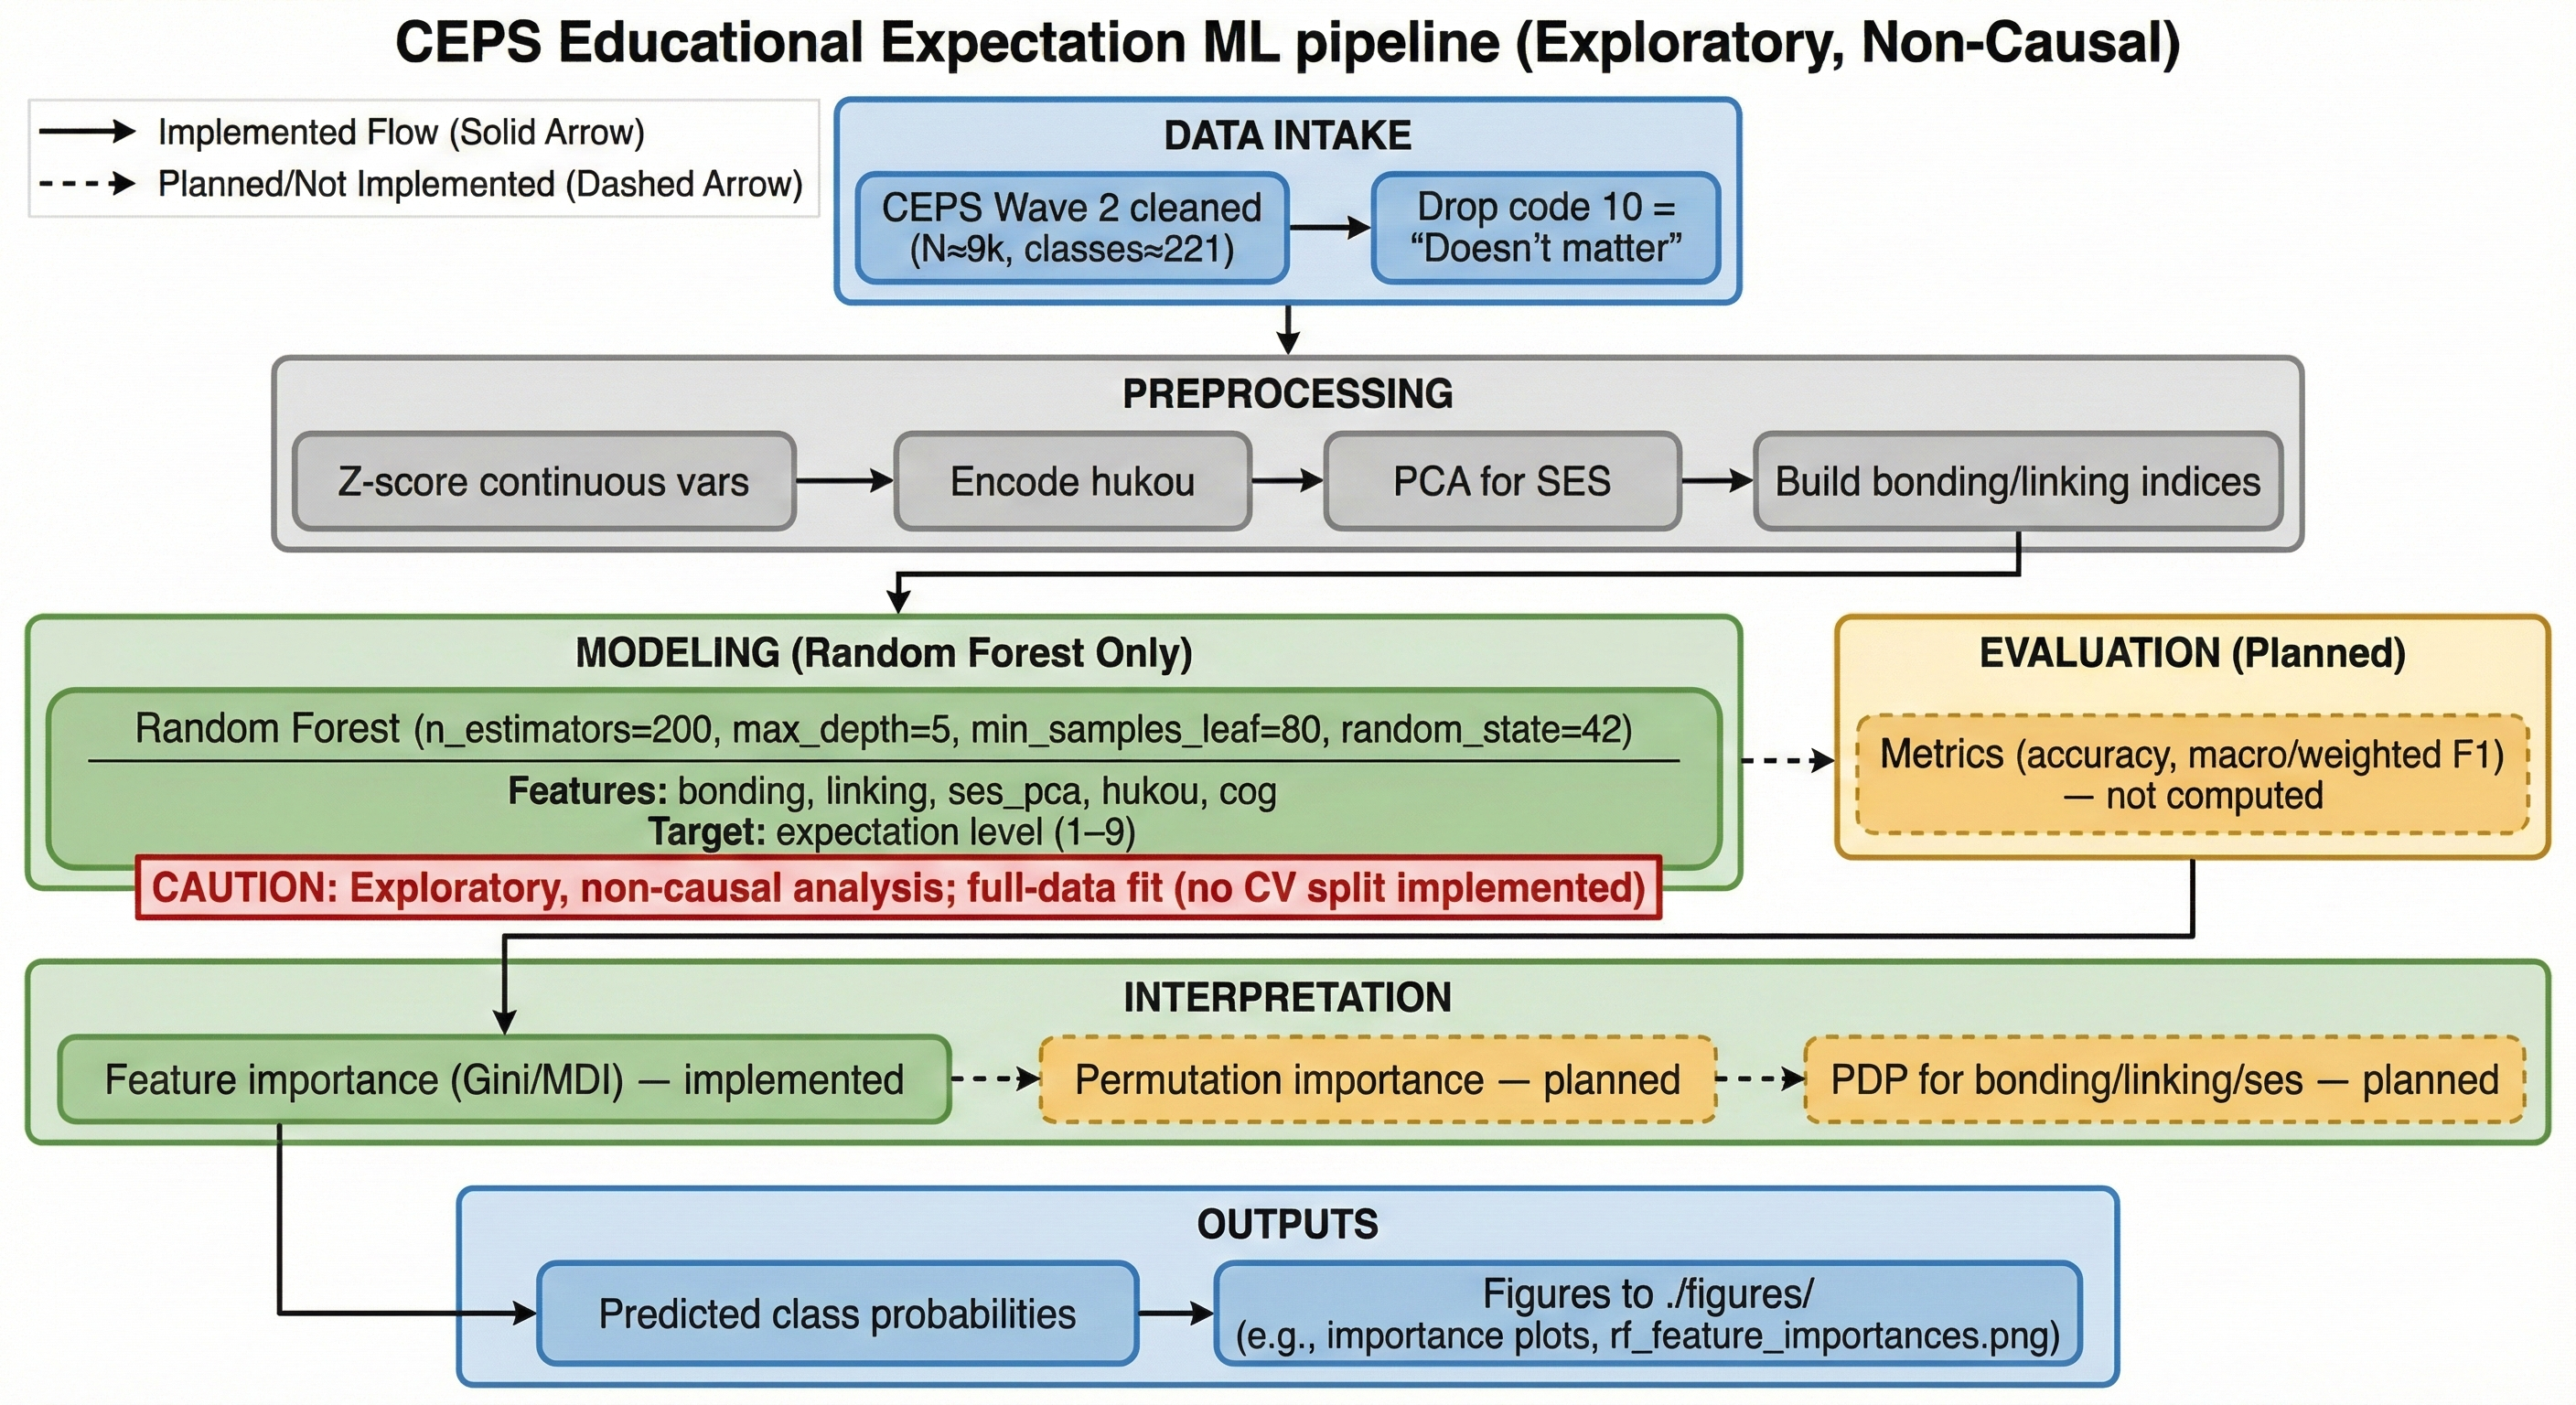
\includegraphics[width=\textwidth]{ml_pipeline.png}
  \caption{机器学习分析流程图:从数据输入到特征重要性输出}
  \label{fig:ml_pipeline}
\end{figure}

\noindent 整个流程可以分为四步:

\paragraph{第一步:准备数据}
\begin{itemize}
    \item 使用与有序 Logit 相同的清洗后数据(约 9,000 名学生)
    \item 剔除"无所谓"选项,保留 1--9 的教育期望等级作为预测目标
    \item 输入变量:同伴关系(Bonding)、师生关系(Linking)、家庭背景(SES)、户籍、认知能力
\end{itemize}

\paragraph{第二步:构建"森林"}
\begin{itemize}
    \item 种植 200 棵决策树
    \item 每棵树最多问 5 层问题(\texttt{max\_depth=5}),防止过于复杂
    \item 每个最终分组至少包含 80 名学生(\texttt{min\_samples\_leaf=80}),确保结论有统计基础
\end{itemize}

\paragraph{第三步:让森林"投票"}
\begin{itemize}
    \item 对每个学生,200 棵树各自给出预测
    \item 汇总所有树的投票,得出最终预测
\end{itemize}

\paragraph{第四步:计算变量重要性}
\begin{itemize}
    \item 统计每个变量在所有树中被用于"提问"的频率和效果
    \item 用得越多、分类效果越好的变量,重要性越高
\end{itemize}

\subsection{变量重要性结果}

图 \ref{fig:rf_importance} 以条形图的形式直观展示了各变量的重要性排名。蓝色条代表本研究关注的学校社会资本变量,灰色条代表控制变量。

\begin{figure}[H]
  \centering
  \includegraphics[width=0.85\textwidth]{../figures/report_phase3/rf_feature_importance.png}
  \caption{随机森林变量重要性条形图:认知能力和家庭 SES 是最强预测因子,学校社会资本(蓝色)贡献约 20\%。}
  \label{fig:rf_importance}
\end{figure}

表 \ref{tab:rf_importance} 列出了具体数值:

\begin{table}[H]
\centering
\caption{随机森林变量重要性排名}
\label{tab:rf_importance}
\begin{tabular}{clc}
\toprule
排名 & 变量 & 重要性得分 \\
\midrule
1 & 认知能力(Cognitive) & 0.409 \\
2 & 家庭社会经济地位(SES) & 0.378 \\
3 & 师生关系(Linking) & 0.133 \\
4 & 同伴关系(Bonding) & 0.070 \\
5 & 户籍类型(Hukou) & 0.010 \\
\bottomrule
\end{tabular}
\vspace{0.5em}

\footnotesize{\textit{注}:重要性得分基于基尼不纯度下降(Gini Impurity Decrease),数值越大表示该变量对预测贡献越大。所有得分加总为 1。}
\end{table}

\subsection{如何解读这个结果?}

\begin{enumerate}
    \item \textbf{认知能力和家庭背景是最强预测因子}:两者合计贡献了近 80\% 的预测能力。这与有序 Logit 的结论一致——学业能力和家庭资源是教育期望的核心决定因素。

    \item \textbf{学校社会资本有独立贡献}:师生关系(13.3\%)和同伴关系(7.0\%)加起来贡献约 20\%。虽然不如认知和 SES 强,但仍是有意义的预测因子。

    \item \textbf{师生关系 $>$ 同伴关系}:这与回归模型中 Linking 系数大于 Bonding 的发现吻合。

    \item \textbf{户籍的独立贡献很小}:仅 1\%。这可能是因为户籍的影响已经被 SES 和认知能力"吸收"了。
\end{enumerate}

\subsection{与有序 Logit 结果的对照}

\begin{table}[H]
\centering
\caption{两种方法结论对比}
\begin{tabular}{lcc}
\toprule
发现 & 有序 Logit & 随机森林 \\
\midrule
认知能力影响最大 & $\checkmark$ (系数最大) & $\checkmark$ (重要性第一) \\
SES 影响显著 & $\checkmark$ & $\checkmark$ (重要性第二) \\
Linking $>$ Bonding & $\checkmark$ (0.19 $>$ 0.14) & $\checkmark$ (0.133 $>$ 0.070) \\
户籍影响较弱 & $\checkmark$ (系数最小) & $\checkmark$ (重要性最低) \\
\bottomrule
\end{tabular}
\vspace{0.5em}

\footnotesize{\textit{结论}:两种方法得出高度一致的结论,增强了研究发现的可信度;同时提醒随机森林未做 hold-out/CV,重要性结果仅作模式对照。}
\end{table}

\subsection{方法局限与注意事项}

\begin{enumerate}
    \item \textbf{这是探索性分析,不是因果证据}:随机森林告诉我们"哪些变量与结果关联更强",但不能证明"改变某个变量会导致结果改变"。

    \item \textbf{没有做训练/测试集划分}:我们用全部数据来训练模型,目的是看整体模式,而不是预测新数据。这意味着模型的预测准确率可能被高估。

    \item \textbf{重要性得分是相对的}:0.409 并不意味着"认知能力解释了 40.9\% 的方差",只是说在这个模型中,认知能力被用得最多、效果最好。
\end{enumerate}

\subsection{数据文件路径}
\begin{itemize}
    \item 输入文件:\texttt{./data/raw/ceps\_w2\_students.dta} (需申请)
    \item 处理后文件:\texttt{./data/processed/merged\_rescued\_all\_with\_pca\_ses.csv}
    \item 回归脚本:\texttt{./analysis/ordinal\_analysis.py}
    \item 随机森林脚本:\texttt{./analysis/ordinal\_rf\_pca.py}(生成特征重要性)
    \item 随机森林出图:\texttt{./analysis/plot\_rf\_importance.py}
\end{itemize}

\subsection{伪代码与命令 (Python/Statsmodels)}

\begin{lstlisting}
# 1. Import Libraries
import pandas as pd
import numpy as np
from statsmodels.miscmodels.ordinal_model import OrderedModel
from sklearn.decomposition import PCA
from sklearn.preprocessing import StandardScaler

# 2. Data Loading & Cleaning
df = pd.read_stata("ceps_w2.dta")
df = df[df['w2b18'] != 10]  # Drop "Doesn't matter"
df['expect_edu'] = df['w2b18'].astype(int)

# 3. Variable Construction (Example: SES PCA)
ses_cols = ['parent_edu_max', 'w2a09', 'w2a13', 'has_desk', 'has_computer']
X_ses = StandardScaler().fit_transform(df[ses_cols].fillna(0)) 
pca = PCA(n_components=1)
df['ses_pca'] = pca.fit_transform(X_ses)
# Final Z-score all continuous vars
for col in ['bonding', 'linking', 'ses_pca', 'cog']:
    df[col] = (df[col] - df[col].mean()) / df[col].std()

# 4. Model Fitting
model = OrderedModel(
    df['expect_edu'],
    df[['linking', 'bonding', 'ses_pca', 'hukou', 'inter_bond_ses']],
    distr='logit'
)
res = model.fit(method='bfgs')

# 5. Clustered Standard Errors
res_clustered = res.get_robustcov_results(cov_type='cluster', groups=df['clsids'])
print(res_clustered.summary())
\end{lstlisting}

\section{结论 (Conclusion)}

\subsection{核心发现}
\begin{enumerate}
    \item \textbf{学校社会资本显著正向预测教育期望}:控制 SES、户籍、认知后,Linking($\beta=0.19$)和 Bonding($\beta=0.14$)均显著($p<0.001$)。

    \item \textbf{师生关系 $>$ 同伴关系}:无论回归系数还是 RF 特征重要性,Linking 的预测力均高于 Bonding。

    \item \textbf{"补偿效应"假设未获支持}:Bonding $\times$ SES 为正($p\approx0.052$),高 SES 学生从同伴关系中获益更多(马太效应);Linking $\times$ SES 不显著,师生关系对不同 SES 群体作用相近。

    \item \textbf{认知与 SES 仍是最强预测因子}:RF 重要性排序为认知(40.9\%)$>$ SES(37.8\%)$>$ Linking(13.3\%)$>$ Bonding(7.0\%)$>$ 户籍(1.0\%)。

    \item \textbf{Linking 存在非线性}:低分段提升效应更强(样条 $p\approx0.005$),改善师生关系对关系较差学生收益更大。

    \item \textbf{两种方法结论一致}:有序 Logit 与随机森林在变量排序和效应方向上高度吻合,增强了结论可信度。
\end{enumerate}

\vspace{0.5em}
\noindent\fbox{\parbox{0.96\textwidth}{
\textbf{一句话总结}:学校社会资本对初中生教育期望有独立正向影响;同伴关系呈马太效应(高 SES 获益更多),师生关系相对公平——政策应优先改善师生关系。
}}

\subsection{研究局限性}

\subsubsection{因果推断局限}
\begin{itemize}
    \item \textbf{横截面数据}:本研究基于单一时点数据,无法排除反向因果(高期望学生可能主动建立更好的社会关系)或遗漏变量偏误(如学生性格、学校质量等未观测因素)。
    \item \textbf{内生性问题}:社会资本变量可能与误差项相关,OLS/有序 Logit 估计可能有偏。
\end{itemize}

\subsubsection{样本选择偏差}
\begin{itemize}
    \item \textbf{剔除"无所谓"群体}:434 名回答"无所谓"的学生被排除,该群体在 SES、认知、社会资本上均显著低于保留样本(t 检验 $p<0.001$)。
    \item \textbf{外推限制}:研究结论仅适用于"有明确升学意愿"的学生群体,不可直接推广至全体初中生。
    \item \textbf{未建模缺失机制}:未采用 Heckman 选择模型或多重插补评估删除样本带来的潜在偏差。
\end{itemize}

\subsubsection{测量局限}
\begin{itemize}
    \item \textbf{自报偏误}:社会资本指标基于学生主观感知(self-reported),缺乏客观的社会网络结构数据(如同伴提名法、社会网络分析)。
    \item \textbf{维度覆盖不全}:Bonding 仅含 3 个条目、Linking 仅含 4 个条目,可能未完全捕捉学校社会资本的丰富内涵。
    \item \textbf{SES 测量}:PCA 方法虽避免多重共线性,但第一主成分仅解释 44.1\% 方差,可能丢失部分信息。
\end{itemize}

\subsubsection{模型假设局限}
\begin{itemize}
    \item \textbf{PO 假设违反}:比例优势假设被显著拒绝($p<0.001$),意味着自变量对不同教育期望阈值的影响系数并非恒定。本研究未实现部分比例优势(Partial PO)模型的正式估计。
    \item \textbf{单层模型}:未采用多层线性模型(HLM)处理班级/学校层级效应,仅通过聚类稳健标准误校正班级内相关性。
    \item \textbf{非线性设定敏感}:Linking 的非线性效应仅在特定样条设定(df=4,degree=3)下成立,稳健性有待进一步验证。
\end{itemize}

\subsubsection{机器学习局限}
\begin{itemize}
    \item \textbf{无交叉验证}:随机森林在全样本上训练,未做 train/test 划分或 k-fold CV,特征重要性可能过拟合。
    \item \textbf{仅作探索性对照}:机器学习结果不具因果含义,仅用于与回归结论交叉验证。
\end{itemize}

\subsection{未来研究方向}

\subsubsection{因果识别策略}
\begin{itemize}
    \item \textbf{追踪数据与固定效应}:利用 CEPS 追踪数据(Wave 1 $\rightarrow$ Wave 2)构建个体固定效应模型,控制不随时间变化的遗漏变量。
    \item \textbf{工具变量法}:寻找影响社会资本但不直接影响教育期望的外生变量(如班级规模、教师流动率)作为工具变量。
    \item \textbf{断点回归/匹配法}:利用政策断点(如户籍改革、学校合并)或倾向得分匹配估计因果效应。
\end{itemize}

\subsubsection{模型拓展}
\begin{itemize}
    \item \textbf{多层模型}:采用 HLM(Hierarchical Linear Model)分离学生层、班级层、学校层的方差成分,检验班级氛围的情境效应(contextual effect)。
    \item \textbf{部分比例优势模型}:对违反 PO 假设的变量允许系数在阈值间变化,更准确刻画异质性效应。
    \item \textbf{广义可加模型(GAM)}:系统检验各自变量的非线性效应,不依赖预设的样条节点。
\end{itemize}

\subsubsection{异质性分析}
\begin{itemize}
    \item \textbf{亚群体比较}:探索社会资本效应在不同群体(留守儿童、流动儿童、重点/普通学校、东/中/西部地区)中的差异。
    \item \textbf{高阶交互}:检验三阶交互(如 Bonding $\times$ SES $\times$ Hukou),探索更复杂的调节机制。
    \item \textbf{分位数回归}:检验社会资本对教育期望分布不同位置(低期望 vs 高期望学生)的差异化影响。
\end{itemize}

\subsubsection{测量改进}
\begin{itemize}
    \item \textbf{社会网络分析}:引入班级提名数据,构建客观网络指标(如度中心性、接近中心性、结构洞)替代自评量表。
    \item \textbf{多维度 Bonding/Linking}:区分情感支持、信息支持、工具支持等不同维度的社会资本作用。
    \item \textbf{Bridging 资本}:纳入跨群体异质性连接指标,构建完整的 Bonding-Bridging-Linking 三维框架。
\end{itemize}

\subsubsection{"无所谓"群体专项研究}
\begin{itemize}
    \item 将回答"无所谓"的学生作为独立研究对象,探究教育"脱嵌"(disengagement)的形成机制。
    \item 采用多项 Logit 或嵌套 Logit 模型,将"无所谓"作为独立类别纳入分析。
    \item 使用 Heckman 选择模型评估样本删除带来的潜在偏差。
\end{itemize}

\subsubsection{机器学习深化}
\begin{itemize}
    \item 加入 k-fold 交叉验证评估模型泛化能力,报告准确率、F1、AUC 等指标。
    \item 生成部分依赖图(PDP)和 SHAP 值,可视化各变量的边际效应和交互作用。
    \item 采用梯度提升(XGBoost/LightGBM)或神经网络作为稳健性对照。
\end{itemize}

\end{document}
